% About
% Dark Beamer theme
%
% Author
% Original author: Blottiere Paul
% Additions: Ioannis Petrousov
%
% Compile
% just run xelatex

% aspect ratio 16:9
\documentclass[12pt,t,aspectratio=169,xcolor=table]{beamer}

% aspect ratio 4:3
% WARNING
% If you decide to use this ration, make sure you adjust the
% position of the date so it sit's exactly on the footer (blue line).
% In general, avoid using this ratio, we 're not in the 90's anymore.
%\documentclass[12pt,t]{beamer}

% usepackage
\usepackage{theme/dbt} % our main theme
\usepackage{algorithm2e}
\usepackage{xltxtra}
\usepackage{xgreek}
\setmainfont[Mapping=tex-text]{GFS Didot}
\usepackage{listings}
\usepackage{multirow} % allows merging cells in tables
\usepackage{hyperref}
\usepackage{caption}

% set color of table caption
\captionsetup[table]{labelfont={color=yellow}}

% set bibliography colors
\setbeamercolor{bibliography item}{fg=white,bg=white}
\setbeamercolor*{bibliography entry title}{fg=white,bg=white}
\setbeamercolor*{bibliography entry author}{fg=keywords,bg=keywords}

% put images in images path
\graphicspath{{images/}}

\title{dark-beamer-theme (DBT)}
\date{Νοέμβριος 2016} % change to the desired date
\subtitle{
Πανεπιστήμιο Δυτικής Μακεδονίας\\
Τμήμα Μηχανικών Πληροφορικής και Τηλεπικοινωνιών
}

\author[me]{Ιωάννης Πετρουσόβ\\[3mm]Επιβλέπων Καθηγητής: Μηνάς Δασυγένης}

\institute {
Εργαστήριο Ψηφιακών Συστημάτων και Αρχιτεκτονικής Υπολογιστών\\
http://arch.icte.uowm.gr
}

\begin{document} {
    \setbeamertemplate{footline}{}
    \frame {
        \titlepage
    }
}

\begin{frame}{Πίνακας περιεχομένων}
\tableofcontents
\end{frame}

\section{Κεφάλαιο 1}
\begin{frame}[plain,c]

\begin{center}
\Huge Τίτλος κεφαλαίου 1
\end{center}

\end{frame}

\begin{frame}
\frametitle{Bullets}
\begin{itemize}
  \setlength\itemsep{1cm}
  \item Ένα
  \item Δύο
  \item Τρία
\end{itemize}
\end{frame}

\begin{frame}{Bullets στήλες}
\begin{columns}[T] % align columns
\begin{column}{.48\textwidth}
\color{red}\rule{\linewidth}{4pt}

Κατηγορία Α
\bigskip
\begin{itemize}
  \setlength\itemsep{0.7cm}
  \item Ένα
  \item Δύο
  \item Τρία
\end{itemize}
\end{column}%
\hfill%
\begin{column}{.48\textwidth}
\color{subtitle}\rule{\linewidth}{4pt}

Κατηγορία Β
\bigskip
\begin{itemize}
  \setlength\itemsep{0.15cm}
  \item Άλφα
  \item Βήτα
  \item Γάμα
\end{itemize}
\end{column}%
\end{columns}
\end{frame}

\section{Κεφάλαιο 2}
\begin{frame}[plain,c]
\begin{center}
\Huge Κεφάλαιο 2
\end{center}
\end{frame}

\begin{frame}{Εικόνες}
\begin{columns}[T] % align columns
\begin{column}{.5\textwidth}

\centering
Αλγόριθμος
	\begin{figure}[h!]
		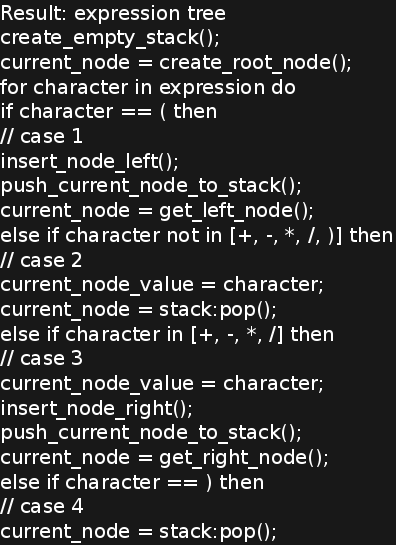
\includegraphics[scale=0.3]{expression_tree_algorithm}
	\end{figure}

\end{column}%
\hfill%
\begin{column}{.5\textwidth}
\centering
$f(x,y)=((2*x)+y)$
\bigskip
	\begin{figure}[h!]
		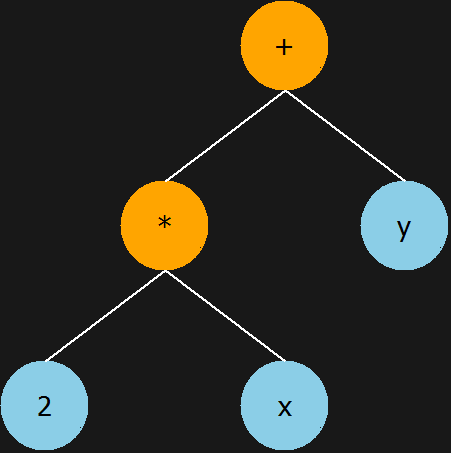
\includegraphics[scale=0.3]{expression_tree_example}
	\end{figure}

\end{column}%
\end{columns}	
\end{frame}

\section{Κεφάλαιο 3}
\begin{frame}[plain,c]
\begin{center}
\Huge Τίτλος κεφαλαίου 3
\end{center}
\end{frame}

\begin{frame}{Μία εικόνα}

	\begin{figure}[h!]
	\vspace*{-1em}
		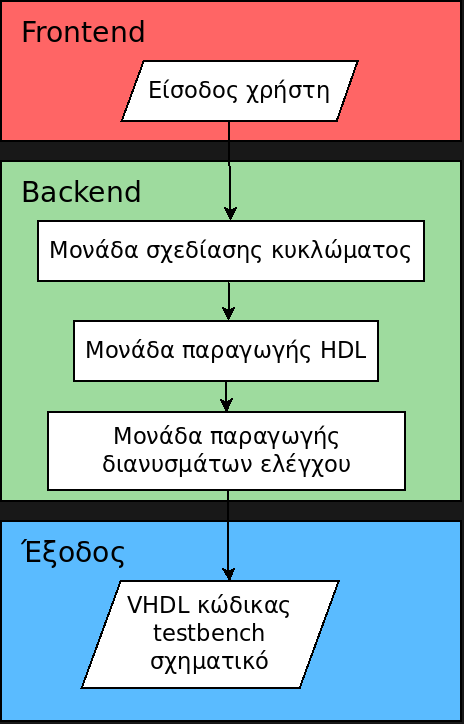
\includegraphics[scale=0.25]{tool_outline}
	\end{figure}
\end{frame}

\begin{frame}[plain,c]
\begin{center}
\Huge Υποκεφάλαιο 1
\end{center}
\end{frame}

\subsection{Υποκεφάλαιο 1}
\begin{frame}[fragile]{Χρήση απεικόνισης}
\begin{itemize}
  \setlength\itemsep{0.15cm}
  \item JSON μορφή
  \item Ένα
  \item Δύο
\end{itemize}
\bigskip
\begin{lstlisting}
{
	"function": "( ( in0 + in1 ) * ( in2 + 73 ) )",
	"in0": 2,
	"in1": 2,
	"in2": 5
}
\end{lstlisting}
\end{frame}

\subsection{Υποκεφάλαιο 2}
\begin{frame}[plain,c]
\begin{center}
\Huge Υποκεφάλαιο 2
\end{center}
\end{frame}

\begin{frame}{Εικόνα με bullets}
\begin{columns}[T] % align columns
\begin{column}{.48\textwidth}
\color{red}\rule{\linewidth}{4pt}
netlist
\bigskip
	\begin{figure}[h!]
	\vspace*{-1em}
		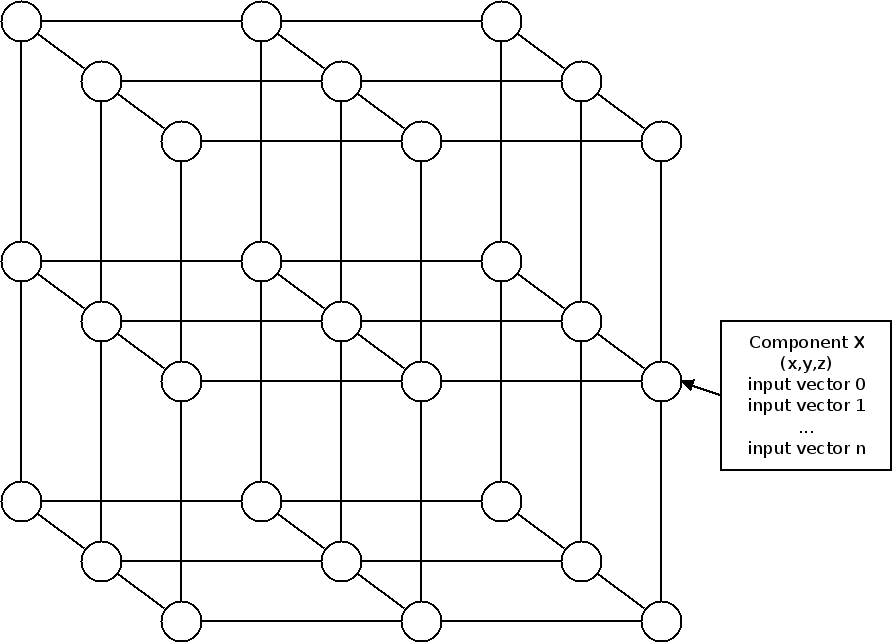
\includegraphics[scale=0.2]{ahdl_hypercube}
	\end{figure}
\end{column}%
\hfill%
\begin{column}{.48\textwidth}
\color{subtitle}\rule{\linewidth}{4pt}

Ιδιότητες
\bigskip
\begin{itemize}
  \setlength\itemsep{0.15cm}
  \item Τρισδιάστατη μορφή
  \item Αποτελείται από 3 δομές
  \begin{itemize}
	  \item components
	  \item interconnections
	  \item componentlist
  \end{itemize}
  \item Δημιουργείται αυτόματα 
\end{itemize}
\end{column}%
\end{columns}	
\end{frame}

\begin{frame}{Χρήση απαρρίθμησης}
%	\setlength\itemsep{0.4cm}
	Παράγει τα διανύσματα ελέγχου που επιβεβαιώνουν την ορθότητα λειτουργίας του κυκλώματος του επιταχυντή
	
	\begin{enumerate}
	\item Πρώτο
	\item Δεύτερο
	\item Τρίτο
	\item Τέταρτο
	\end{enumerate}

\bigskip
Παράδειγμα testbench της συνάρτηση $f(x,y)=x+y$

%	\begin{figure}[h!]
%	\vspace*{-1em}
%	\bigskip
%	\begin{center}
%	\hspace*{-11mm}
%	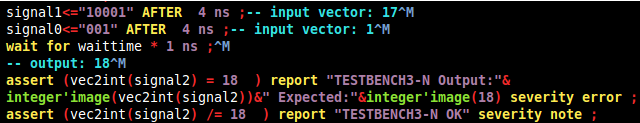
\includegraphics[keepaspectratio=true,width=16cm]{tb}
	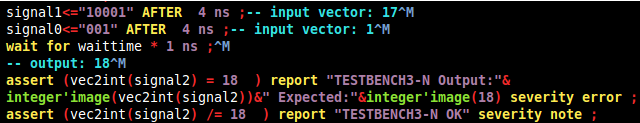
\includegraphics[scale=0.6]{tb}
%	\end{center}
%	\end{figure}

\end{frame}

\begin{frame}{Bullets γραμμές}
	\begin{itemize}
	\item Κατηγορία Α1
	\item Κατηγορία Α2
	\end{itemize}

\bigskip

Προαιρετικά:
	\begin{itemize}
		\item Κατηγορία Β1
		\item Κατηγορία Β2
	\end{itemize}
\end{frame}

\section{Χρήση πίνακα}
\begin{frame}{Παράδειγμα πίνακα}
\begin{table}[]
\centering
\caption{My caption}
\label{my-label}
\begin{tabular}{|ccccc|}
\hline
bits & type1 & type2 & slices & \begin{tabular}[c]{@{}c@{}}freq\\ (MHZ)\end{tabular} \\ \hline
8    & 4     & 3     & 4      & 351.864                                              \\ \hline
16   & 8     & 7     & 9      & 286.697                                              \\ \hline
32   & 16    & 15    & 24     & 229.252                                              \\ \hline
64   & 32    & 31    & 42     & 207.468                                              \\ \hline
128  & 64    & 63    & 96     & 181.917                                              \\ \hline
\end{tabular}
\end{table}
\end{frame}

\section{Επίδειξη λειτουργίας}
\begin{frame}[plain,c]{Επίδειξη λειτουργίας}
\begin{center}
\large\url{http://arch.icte.uowm.gr/hdl/equationparser_json.php}
\end{center}
\end{frame}


\begin{frame}[plain,c]
\begin{center}
\Huge Ευχαριστώ\\για την προσοχή σας
\color{title}\small\vfill petrousov@gmail.com\\
\url{http://petrousov.net/}
\small\vfill\url{http://arch.icte.uowm.gr/hdl/equationparser_json.php}
\end{center}
\end{frame}




\end{document}